\PassOptionsToPackage{spanish}{translator}
\documentclass{beamer} %handout, notes=show

\usepackage[spanish, es-tabla]{babel}

%\uselanguage{spanish}
%\languagepath{spanish}

%\deftranslation[to=spanish]{Example}{Ejemplo}
%\deftranslation[to=spanish]{example}{ejemplo}

\mode<presentation> {

% The Beamer class comes with a number of default slide themes
% which change the colors and layouts of slides. Below this is a list
% of all the themes, uncomment each in turn to see what they look like.

%\usetheme{default}
%\usetheme{AnnArbor}
%\usetheme{Antibes}
%\usetheme{Bergen}
%\usetheme{Berkeley}
%\usetheme{Berlin}
%\usetheme{Boadilla}
%\usetheme{CambridgeUS}
%\usetheme{Copenhagen}
%\usetheme{Darmstadt}
%\usetheme{Dresden}
%\usetheme{Frankfurt}
%\usetheme{Goettingen}
%\usetheme{Hannover}
%\usetheme{Ilmenau}
%\usetheme{JuanLesPins}
%\usetheme{Luebeck}
\usetheme{Madrid}
%\usetheme{Malmoe}
%\usetheme{Marburg}
%\usetheme{Montpellier}
%\usetheme{PaloAlto}
%\usetheme{Pittsburgh}
%\usetheme{Rochester}
%\usetheme{Singapore}
%\usetheme{Szeged}
%\usetheme{Warsaw}

% As well as themes, the Beamer class has a number of color themes
% for any slide theme. Uncomment each of these in turn to see how it
% changes the colors of your current slide theme.

%\usecolortheme{albatross}
%\usecolortheme{beaver}
%\usecolortheme{beetle}
%\usecolortheme{crane}
%\usecolortheme{dolphin}
%\usecolortheme{dove}
%\usecolortheme{fly}
%\usecolortheme{lily}
%\usecolortheme{orchid}
%\usecolortheme{rose}
%\usecolortheme{seagull}
%\usecolortheme{seahorse}
%\usecolortheme{whale
%\usecolortheme{wolverine}

%\setbeamertemplate{footline} % To remove the footer line in all slides uncomment this line
%\setbeamertemplate{footline}[page number] % To replace the footer line in all slides with a simple slide count uncomment this line

%\setbeamertemplate{navigation symbols}{} % To remove the navigation symbols from the bottom of all slides uncomment this line
}

\usepackage[utf8]{inputenc}
\usepackage{amsmath}
\usepackage{graphicx}
\usepackage{booktabs} % Allows the use of \toprule, \midrule and \bottomrule in tables
\usepackage{multicol}

\usepackage[export]{adjustbox} % Para bordes en las imágenes.

\usepackage{svg}

\setkeys{Gin}{height=7cm}

\graphicspath{{imagenes/}}

\DeclareMathOperator*{\argmax}{arg\,max}

% \AtBeginSubsection{
%     \begin{frame}
%         \frametitle{Índice de contenido}
%         \begin{multicols}{2}
%             \tableofcontents[currentsubsection]
%         \end{multicols}
%     \end{frame}
% }

\AtBeginSection{
    \begin{frame}
        \frametitle{Índice de contenido}
        \begin{multicols}{2}
            \tableofcontents[currentsection]
        \end{multicols}
    \end{frame}
}

\title[Detección de humor]{Detección de humor en textos en español}

\author{Santiago \textsc{Castro} --- Matías \textsc{Cubero}}
\institute[]{
    Facultad de Ingeniería, Universidad de la República \\
    \medskip
    \textit{sacastro@fing.edu.uy --- mcubero@fing.edu.uy}
}
\date{\today}

\begin{document}

\begin{frame}
    \titlepage
\end{frame}

\begin{frame}[shrink]{Outline}
    \frametitle{Índice de Contenido}
    \begin{multicols}{2}
        \tableofcontents
    \end{multicols}
\end{frame}

\section{Introducción} 

\subsection{Motivación}

\begin{frame}[allowframebreaks]
    \frametitle{Motivación}
    \begin{itemize}
        \item La risa caracteriza al ser humano como especie.
        \item Componente esencial en la comunicación humana.
        \item Humor como pieza fundamental en la interacción persona-computadora.
    \end{itemize}

    \framebreak
    
    \begin{itemize}
        \item El humor ha sido estudiado desde el punto de vista psicológico, cognitivo y lingüístico.
        \item ¿Pero desde el punto de vista computaciónal?
    \end{itemize}
    Algunos trabajos previos existen, pero se está aún lejos de concretar una caracterización del humor que permita su reconocimiento y generación automática.
\end{frame}

\subsection{Objetivos}

\begin{frame}
    \frametitle{Objetivos}
    \begin{itemize}
        \item Construir un clasificador de humor en textos en español utilizando métodos de aprendizaje automático
            \begin{itemize}
                \item En particular en tweets
            \end{itemize}
        \item Construir un corpus de tweets en español
    \end{itemize}
\end{frame}


\begin{frame}
    \frametitle{Dificultad}
    El 28 de diciembre del 2012 van a salir los mayas a decir: ``¡Feliz día de los inocentes!''
\end{frame}

\section{Estado del arte}

\subsection{Definiciones}
\begin{frame}[allowframebreaks]
    \frametitle{Definiciones}

    \begin{block}{Humor $\not\subset$ Gracioso}
        Modo de presentar, enjuiciar o comentar la realidad, resaltando el lado cómico, risueño o ridículo de las cosas.  
    \end{block}
    \begin{block}{Chiste $\subset$ Humor}
        Dicho u ocurrencia graciosa.
    \end{block}

    \framebreak

    \begin{block}{Ironía}
        Figura retórica que consiste en dar a entender lo contrario a lo que se dice.
    \end{block}
    \begin{block}{Sátira}
        Composición en verso o prosa cuyo objetivo es censurar o ridiculizar a alguien o algo
    \end{block}
    \begin{block}{Sarcasmo}
        Burla sangrienta, ironía mordaz y cruel con que se ofende o maltrata a alguien o algo.
    \end{block}
    \begin{block}{Ingenio}
        Chispa, talento para ver y mostrar rápidamente el aspecto gracioso de las cosas.
    \end{block}

    \framebreak
        
    \begin{eqnarray*} %% Do avoid eqnarray if possible.
        \text{humor} \iff&  \text{cómico} \\
        \text{ironía} \iff& \text{significar lo contrario} \\
        \text{sátira} \iff& \text{crítica + humor} \\
        \text{sarcasmo} \iff& \text{burla} \\
        \text{ingenio}  \iff& \text{perspicacia en el humor}
    \end{eqnarray*}
\end{frame}

\subsection{Teorías}
\begin{frame}
    \frametitle{Teoría de la superioridad}

    \textbf{Superioridad}: siempre nos reímos de alguien. (risa = ganar)
    \begin{example}
        — ¿En qué se parece Superman a un político honesto? \\
        — En que ninguno de los dos existe.
    \end{example}
\end{frame}

\begin{frame}
\frametitle{Teoría del alivio}
    \textbf{Aliviarse}: de temas que generan tensión, como el sexo, la muerte, etc.
    \begin{example}
        —Bienvenida a McDonald’s, ¿qué le doy?\\
        —¡Vergüenza!\\
        —¡Mamá! ¡Estoy trabajando!\\
        —Uy, perdóneme ``señor licenciado en diseño gráfico''\\
    \end{example}
\end{frame}

\begin{frame}
\frametitle{Teoría de la resolución de incongruencias}
    \textbf{Resolución de incongruencia}: percepción repentina de conflicto cognitivo, encontrando luego un sentido
    \begin{example}
        — Mi amor llevamos 30 años juntos, ¿por qué no nos casamos?\\
        — Mejor no, ¿quién se va a querer casar con nosotros?
    \end{example}
\end{frame}

\begin{frame}
\frametitle{Teoría de la violación}
    \textbf{Violación}: de cómo pienso que van a ser las cosas, aunque la situación parece normal
    \begin{example}
        Mi iPhone 6 Plus lo cuido tanto que todavía está en su caja. . . en la tienda. . . en el shopping. . .
    \end{example}
\end{frame}

\begin{frame}
\frametitle{Teorías sociológicas}
    \begin{itemize}
        \item Fines sociológicos de mantenimiento
        \item Fines sociológicos de negociación
        \item Fines sociológicos de cambio de contexto
    \end{itemize}
\end{frame}

\begin{frame}
\frametitle{Teoría de los guiones semánticos del humor}
    Oposición de guiones semánticos
    \begin{example}
        Él rompió su corazón. Ella rompió su PlayStation 4. Creo que todos sabemos quién lloró más fuerte.
    \end{example}
\end{frame}

\begin{frame}
\frametitle{Teoría general del humor verbal}
    Respuesta innovadora y familiar a un estímulo
    \begin{example}
        — Cariño, dame el bebé.\\
        — Espera a que llore.\\
        — ¿A que llore?. ¿Por qué?\\
        — ¡Porque no lo encuentro!\\
    \end{example}
\end{frame}

\subsection{Enfoques computacionales}
\begin{frame}
\frametitle{Enfoques Computaciones}
    \begin{itemize}
        \item Existen dos trabajos similares a este proyecto.
        \begin{itemize}
            \item Making Computers Laugh: Investigations in Automatic Humor Recognition, Mihalcea y Strapparava (2005)
            \item Recognizing Humor Without Recognizing Meaning, Sjöbergh y Araki (2007)
        \end{itemize}
        \item Ambos implementan características que cumplen los textos de humor para poder detectarlos
        \item Existen otros trabajos donde se enfoca a estudiar una característica del humor sin tener como fin detectarlo.
    \end{itemize}
\end{frame}

% \subsubsection{Características}
\begin{frame}
\frametitle{Aliteración}
    Repetición notoria del mismo o de los mismos fonemas, sobre todo consonánticos, en una frase.
    \begin{example}
        Cuando pasé por tu puerta me tiraste una flor, la próxima vez que pase, ¡sin maceta por favor!
    \end{example}
\end{frame}

\begin{frame}
\frametitle{Antonímia}
    La antonimia es la relación de oposición entre los significados de dos palabras (útil — inútil)
    \begin{example}
        — ¿Qué le dice Tarzán a un ratón?\\
        — ¡Tan pequeño y con bigote!\\
        — ¿Y qué le dice el ratón a Tarzán?\\
        — ¡Tan grandote y con pañal!\\
    \end{example}
\end{frame}

\begin{frame}
\frametitle{Ambigüedad}
    De las palabras y de la oración
    \begin{example}
        La perra de mi vecina me ladró.
    \end{example}
\end{frame}

\begin{frame}
\frametitle{Negatividad}
    El humor tiene una tendencia hacia las connotaciones negativas
    \begin{example}
        — Dr., ¿cómo hago para vivir 100 años?\\
        — Nada de sexo, alcohol ni vicios.\\
        — ¿Y funciona?\\
        — No sé, pero seguro que se le va a hacer largo.
    \end{example}
\end{frame}

\begin{frame}
\frametitle{Jerga Sexual}
    El humor basado en jerga adulta es altamente popular
    \begin{example}
        — Che, ¿qué significa “let’s fuck”?\\
        — Tengamos sexo.\\
        — Bueno, pero después me decís qué significa.
    \end{example}
\end{frame}

\begin{frame}
\frametitle{Palabras Clave}
    Hay palabras que son más mencionadas en textos de humor que en textos de no humor, y viceversa.
    \begin{example}
        -Mamá, ¡en la escuela me dicen Superman!\\
        -Ay Jaimito, ¡otra vez te pusiste los calzoncillos encima de los pantalones!
    \end{example}
\end{frame}

\begin{frame}
\frametitle{Centrado en personas}
    \begin{itemize}
        \item Constantemente referenciando a escenarios relacionados con personas
        \item Palabras como “tú”, “yo”, etc.
    \end{itemize}
\end{frame}

\begin{frame}
\frametitle{Perplejidad - OOV}
    \begin{itemize}
        \item Se construye un modelo del lenguaje a partir de narraciones
        \item La perplejidad en textos de humor es mayor
        \item Más frecuente encontrar palabras OOV en textos de humor
    \end{itemize}
\end{frame}

\begin{frame}
\frametitle{Making Computers Laugh}
    \begin{itemize}
        \item Utilizan: aliteración, antonimia y jerga sexual.
        \item Precisión: 96,95\% Reuters, 79,15\% BNC y 84,82\% proverbios.
    \end{itemize}
\end{frame}

\begin{frame}
\frametitle{Recognizing Humor Without Recognizing Meaning}
    \begin{itemize}
        \item Utilizan: palabras claves, ambigüedad, aliteración, antonimia y palabras centradas en las personas.
        \item Precisión: 85,4\%.
    \end{itemize}
\end{frame}

\section{Construcción del corpus}

\subsection{Extracción}
\begin{frame}
    \frametitle{Extracción}

    \begin{itemize}
        \item Humorístico: se busca en Twitter por la palabra clave \emph{chistes} y se eligen cuentas, llegando a 16.488 tweets.
        \item No humorístico: cuentas de noticias, frases filosóficas y curiosidades, alcanzando los 22.875 tweets.
    \end{itemize}
\end{frame}

\subsection{Anotación}
\begin{frame}[allowframebreaks]
    \frametitle{Anotación}

    \begin{itemize}
        \item Naturalmente se etiquetarían los tweets según su tipo de cuenta; pero se encuentran inconsistencias.

        \begin{itemize}
            \item Hay que anotarlos a mano.
        \end{itemize}

        \item Excesiva cantidad de tweets para anotar.

        \begin{itemize}
            \item Se crea una aplicación para que usuarios los anoten.
        \end{itemize}
    \end{itemize}

    \vspace{1cm}

    \begin{center}
        \bf
        Los usuarios definen al humor.
    \end{center}

    \framebreak

    \begin{itemize}
        \item Cantidad de clases a considerar
        \item Contenido explícito
        \item Eficiencia
        \item Algoritmo de selección
    \end{itemize}

    \framebreak

    \begin{center}
        \begin{columns}[c]
            \begin{column}[c]{0.45\textwidth}
                \centering
                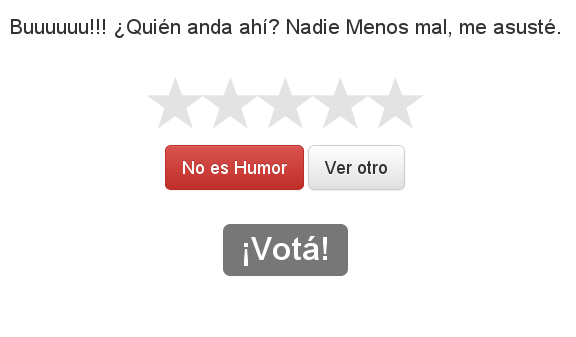
\includegraphics[frame, height=3.5cm]{pagina.png}
            \end{column}

            \begin{column}[c]{0.45\textwidth}
                \centering
                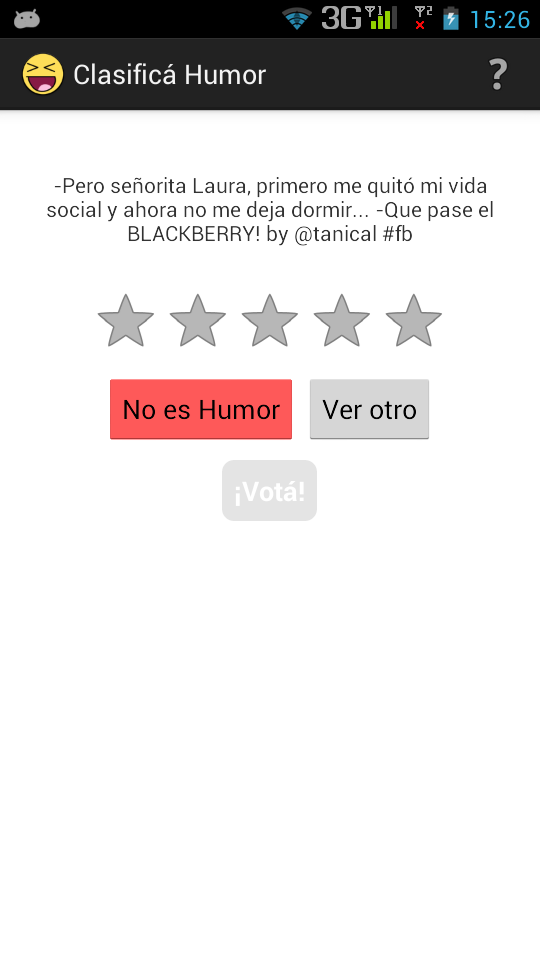
\includegraphics[frame, height=7cm]{app.png}
            \end{column}
        \end{columns}
    \end{center}
\end{frame}

\subsubsection{Resultado de la anotación}
\begin{frame}[allowframebreaks]
    \frametitle{Resultado de la anotación}

    \begin{itemize}
        \item[+] 60k votaciones recibidas
        \item[--] 20k votaciones eliminadas
        \item[--] 6,5k votaciones “ver otro” (\emph{“skip”})
        \item[=] 33,5k votos considerados
    \end{itemize}

    \framebreak

    \begin{center}
        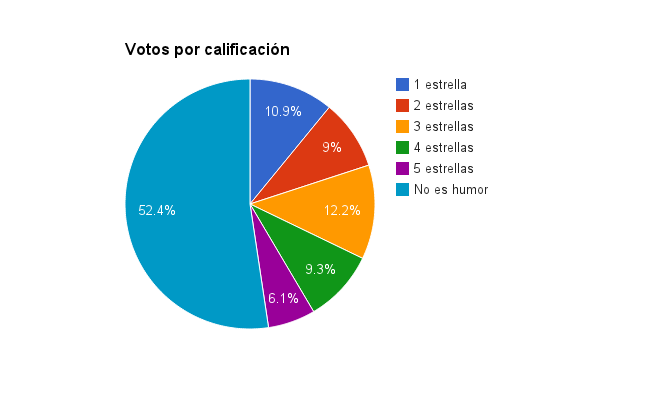
\includegraphics{votos_por_calificacion_torta.png}

        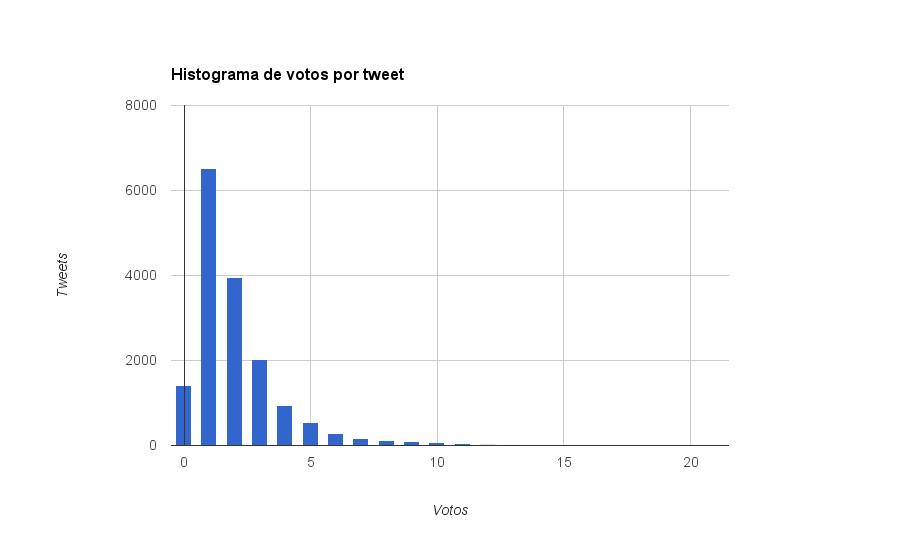
\includegraphics{histograma.png}
    \end{center}
\end{frame}

\subsubsection{Humor según la votación}

\begin{frame}[allowframebreaks]
    \frametitle{Humor según la votación}

    Porcentaje de votos positivos: $\frac{\#\{votos\ positivos\}}{\#\{total\ votos\}}$

    \begin{center}
        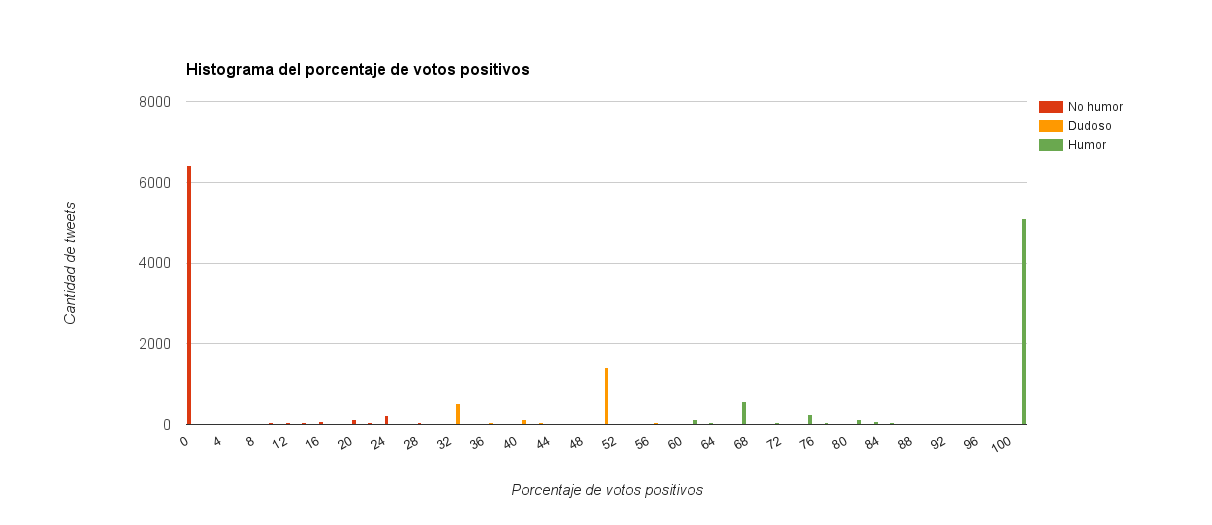
\includegraphics[height=3.75cm]{histograma_porcentaje_humor.png}
    \end{center}

    \begin{itemize}
        \item $[60\%, 100\%] \Rightarrow$ \textbf{Humor}
        \item $(30\%, 60\%) \Rightarrow$ \textbf{Dudoso}
        \item $[0\%, 30\%] \Rightarrow$ \textbf{No humor}
    \end{itemize}

    \framebreak

    \begin{center}
        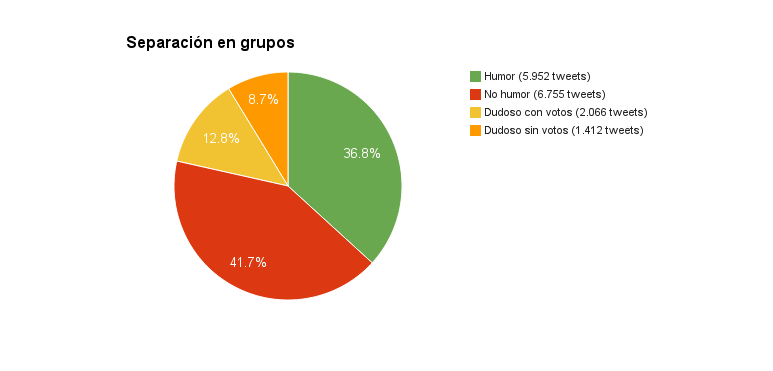
\includegraphics[height=6.5cm]{grupos.png}
    \end{center}
\end{frame}

\subsubsection{Concordancia entre los anotadores}

\begin{frame}[allowframebreaks]
    \frametitle{Concordancia entre los anotadores}

    \begin{itemize}
        \item Se quiere saber qué tan de acuerdo estuvieron las personas a la hora de votar.
        \item Se utiliza la medida kappa de Fleiss.
        \item kappa evalúa cuán mejor es la votación respecto a una al azar, siendo lo mejor posible 1 y siendo 0 una votación al azar.
    \end{itemize}

    \framebreak

    \begin{center}
        \begin{tabular}{ c | r | c }
            tweets considerados & \#tweets & $\kappa$ \\
            \hline
            $\geq$2 votos & 8.320 & 0,612 \\
            $\geq$3 votos & 4.309 & 0,523 \\
            $\geq$4 votos & 2.273 & 0,469 \\
            $\geq$5 votos & 1.331 & 0,434 \\
            $\geq$6 votos & 805 & 0,406 \\
            $\geq$7 votos & 527 & 0,388 \\
            $\geq$8 votos & 354 & 0,381 \\
            $\geq$9 votos & 244 & 0,359 \\
            $\geq$10 votos & 164 & 0,323 \\
            $\geq$11 votos & 105 & 0,309 \\
            $\geq$12 votos & 64 & 0,293 \\
        \end{tabular}

        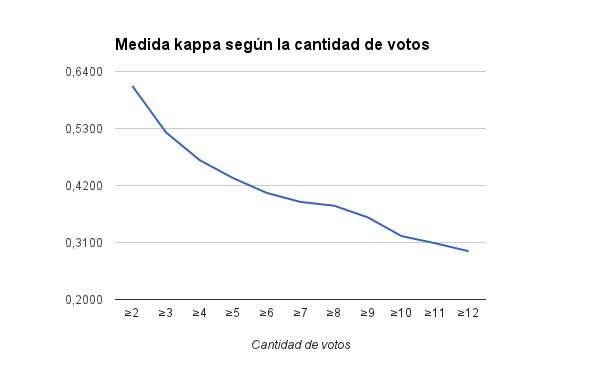
\includegraphics{kappa.png}
    \end{center}

    \framebreak

    \begin{itemize}
        \item \large{0,612; acuerdo de nivel \textbf{medio-alto}}
    \end{itemize}
\end{frame}

\section{Aprendizaje Automático}

\subsection{Clasificadores}
\begin{frame}
    \frametitle{Paragraphs of Text}
    Clasificadores
\end{frame}

\subsection{Métricas}
\begin{frame}
    \frametitle{Paragraphs of Text}
    Métricas
\end{frame}

\section{Clasificador}

\subsection{Metodología}
\begin{frame}
    \frametitle{Metodología}

    \begin{itemize}
        \item Se utilizan SVM, kNN, DT, GNB y MNB.
        \item Se divide en 80\% entrenamiento y 20\% evaluación.
        \item Se usa validación cruzada sobre el conjunto de entrenamiento para resultados intermedios durante el desarollo y el conjunto de evaluación para el resultado final.
    \end{itemize}
\end{frame}
\note{
    Se usa el conjunto de evaluación al final para no sesgarse demasiado a los resultados.
}

\subsection{Línea base}
\begin{frame}
    \frametitle{Línea base}

    \begin{enumerate}
        \item BoW + MNB

        \item Clasificador que predice según lo que dice la mayoría (Negativo)
    \end{enumerate}

    \begin{center}
        \scriptsize
        \begin{tabular}{ c | r | r | r | r | r | r | r }
            & \multicolumn{1}{c |}{Precisión} & \multicolumn{1}{c |}{Recall} & \multicolumn{1}{c |}{$F_1$} & \multicolumn{1}{c |}{Prec. neg.} & \multicolumn{1}{c |}{Rec. neg.} & \multicolumn{1}{c |}{$F_1$ neg.} & \multicolumn{1}{c}{Acierto} \\
            \hline
            LB1 & \textbf{65,2} & \textbf{82,7} & \textbf{72,9} & \textbf{96,3} & 91,2 & \textbf{93,7} & \textbf{89,7} \\
            \hline
            LB2 & N/A & 0,0 & N/A & 82,5 & \textbf{100,0} & 90,4 & 82,5 \\
        \end{tabular}
    \end{center}
\end{frame}

\subsection{Características}

\begin{frame}
    \frametitle{Características}

    Qué se busca:

    \begin{itemize}
        \item Contradicción y negatividad
        \item Formato
        \item Informalidad
        \item Orientación en personas
        \item Temas recurrentes en chistes
    \end{itemize}
\end{frame}

\begin{frame}
    \frametitle{Contradicción y negatividad}
    \framesubtitle{Antónimos}

    \begin{itemize}
        \item Cantidad de pares de antónimos en el tweet:
    \end{itemize}

    \begin{center}
        \[
            Antonimos(tweet) = \frac{|\{pares\ de\ antonimos\}|}{\sqrt{|tweet|}}
        \]
    \end{center}
\end{frame}

\begin{frame}
    \frametitle{Contradicción y negatividad}
    \framesubtitle{Negación}

    \begin{itemize}
        \item Cantidad de ``no'' en el tweet
    \end{itemize}
\end{frame}

\begin{frame}
    \frametitle{Formato}
    \framesubtitle{Diálogo}

    \begin{itemize}
        \item Si el tweet es un diálogo o no
    \end{itemize}
\end{frame}

\begin{frame}
    \frametitle{Formato}
    \framesubtitle{Links}

    \begin{itemize}
        \item Cantidad de hipervínculos en el tweet
    \end{itemize}
\end{frame}

\begin{frame}
    \frametitle{Formato}
    \framesubtitle{Preguntas-respuestas}

    \begin{itemize}
        \item Cantidad de preguntas seguidas de respuestas en el tweet.
    \end{itemize}
\end{frame}

\begin{frame}
    \frametitle{Informalidad}
    \framesubtitle{Exclamación}

    \begin{itemize}
        \item Cantidad de signos de exclamación:
    \end{itemize}

    \begin{center}
        \[
            Exclamacion(tweet) = \frac{|\{signos\ de\ exclamacion\}|}{\sqrt{|tweet|}}
        \]
    \end{center}
\end{frame}

\begin{frame}
    \frametitle{Informalidad}
    \framesubtitle{Hashtags}

    \begin{itemize}
        \item Cantidad de hashtags en el tweet
    \end{itemize}
\end{frame}

\begin{frame}
    \frametitle{Informalidad}
    \framesubtitle{Palabras fuera del vocabluario (OOV)}

    \begin{itemize}
        \item Cantidad de palabras fuera del vocabulario, dividido entre el total
        \item Son varias características:
        \begin{itemize}
            \item Freeling
            \item Freeling-Google
            \item Freeling-Wiktionary
            \item Wiktionary
        \end{itemize}
    \end{itemize}
\end{frame}
\note{
    Las distintas combinaciones de vocabulario debido a costo de uso y debido a ventajas y desventajas de cada uno. \textbf{Freeling} el más barato de usar, offline. Tiene un español más clasico, pero no tiene palabras ``nuevas''. \textbf{Wiktionary} tiene un término medio de todo. Es online, pero no limita su uso. Con \textbf{Google} se pueden obtener muchas palabras ``nuevas'' (como iPhone) y también detección de errores ortográficos, pero limita su uso.
}

\begin{frame}
    \frametitle{Informalidad}
    \framesubtitle{Palabras mayúsculas}

    \begin{itemize}
        \item Cantidad de palabras totalmente en mayúsculas:
    \end{itemize}

    \begin{center}
        \[
            PalabrasMayusculas(tweet) = \frac{|\{palabras\ mayusculas\}|}{\sqrt{|tweet|}}
        \]
    \end{center}
\end{frame}

\begin{frame}
    \frametitle{Informalidad}
    \framesubtitle{Palabras no españolas}

    \begin{itemize}
        \item Cantidad de palabras que tienen caracteres fuera del alfabeto español, normalizado según el total.
    \end{itemize}
\end{frame}

\begin{frame}
    \frametitle{Orientado a personas}
    \framesubtitle{Primera y segunda persona}

    \begin{itemize}
        \item Se busca por palabras flexionadas en primera persona y se hace lo mismo con segunda persona
    \end{itemize}
\end{frame}

\begin{frame}
    \frametitle{Temas recurrentes en chistes}
    \framesubtitle{Distancia temática}

    \begin{itemize}
        \item Cercanía a una categoría de chiste de Chistes.com o cercanía a una oración de la Wikipedia.
        \item BoW + MNB
        \item Categorías
        \begin{itemize}
            \item Chistes cortos
            \item Adivinanzas
            \item Animales
            \item Atlantes
            \item Otros...
        \end{itemize}
    \end{itemize}
\end{frame}
\note{TODO: Aclarar qué es atlantes.}

\begin{frame}
    \frametitle{Temas recurrentes en chistes}
    \framesubtitle{Jerga sexual}

    \begin{itemize}
        \item Se arma un diccionario de jerga sexual mediante \emph{Bootstrapping} en Twitter.
        \item Intersección de multiconjuntos:
    \end{itemize}

    \begin{center}
        \[
            JergaSexual(tweet) = \frac{|tweet \cap DIC_{JS}|}{\sqrt{|tweet|}}
        \]
    \end{center}
\end{frame}

\begin{frame}
    \frametitle{Temas recurrentes en chistes}
    \framesubtitle{Palabras clave}

    \begin{itemize}
        \item Lista de palabras frecuentes en tweets
        \item Intersección de multiconjuntos:
    \end{itemize}

    \begin{center}
        \[
            PalabrasClave(tweet) = \frac{|tweet \cap DIC_{PF}|}{\sqrt{|tweet|}}
        \]
    \end{center}
\end{frame}

\begin{frame}
    \frametitle{Temas recurrentes en chistes}
    \framesubtitle{Presencia de animales}

    \begin{itemize}
        \item Se conforma una lista de animales a partir de los chistes de animales de Chistes.com ($DIC_A$)
        \item Intersección de multiconjuntos:
    \end{itemize}

    \begin{center}
        \[
            PresenciaAnimales(tweet) = \frac{|tweet \cap DIC_A|}{\sqrt{|tweet|}}
        \]
    \end{center}
\end{frame}
\note{
    Características simples.
    $tweet$ es visto como una lista de tokens.
    En general todas las featuers se normalizan según el largo del tweet en tokens, para no sesgar.
}

\subsection{Selección de características}
\begin{frame}[allowframebreaks]
    \frametitle{Selección de características}

    \begin{itemize}
        \item ExtraTrees es usado para hacer un ranking de características.
        \item Se utiliza la Eliminación recursiva de atributos para seleccionar aquellos relevantes y no redundantes.
    \end{itemize}

    \framebreak

    ExtraTrees:

    \begin{center}
        \tiny
        \begin{tabular}{ c | r }
            \multicolumn{1}{c |}{\textbf{Característica}} & \multicolumn{1}{c}{\textbf{Valor}} \\
            \hline
            CLASE & 74,05 \\
            \hline
            Diálogo & 10,86 \\
            \hline
            Distancia temática: Otros... & 03,07 \\
            \hline
            Distancia temática: Atlantes & 02,65 \\
            \hline
            Distancia temática: Chistes cortos & 02,53 \\
            \hline
            Preguntas-respuestas & 01,98 \\
            \hline
            Distancia temática: Adivinanzas & 0,95 \\
            \hline
            Distancia temática: Animales & 0,87 \\
            \hline
            Palabras clave & 0,57 \\
            \hline
            Exclamación & 0,57 \\
            \hline
            Hashtags & 0,55 \\
            \hline
            Links & 0,54 \\
            \hline
            Primera persona & 0,21 \\
            \hline
            Segunda persona & 0,15 \\
            \hline
            OOV Freeling & 0,08 \\
            \hline
            Palabras mayúsculas & 0,06 \\
            \hline
            ALEATORIA & 0,06 \\
            \hline
            Jerga sexual & 0,06 \\
            \hline
            Negación & 0,05 \\
            \hline
            OOV Wiktionary & 0,04 \\
            \hline
            OOV Freeling Wiktionary & 0,03 \\
            \hline
            Presencia de animales & 0,03 \\
            \hline
            OOV Freeling Google & 0,03 \\
            \hline
            Antónimos & 0,02 \\
            \hline
            Palabras no españolas & 0,00 \\
        \end{tabular}
    \end{center}

    \framebreak

    Eliminación recursiva de atributos:

    \begin{center}
        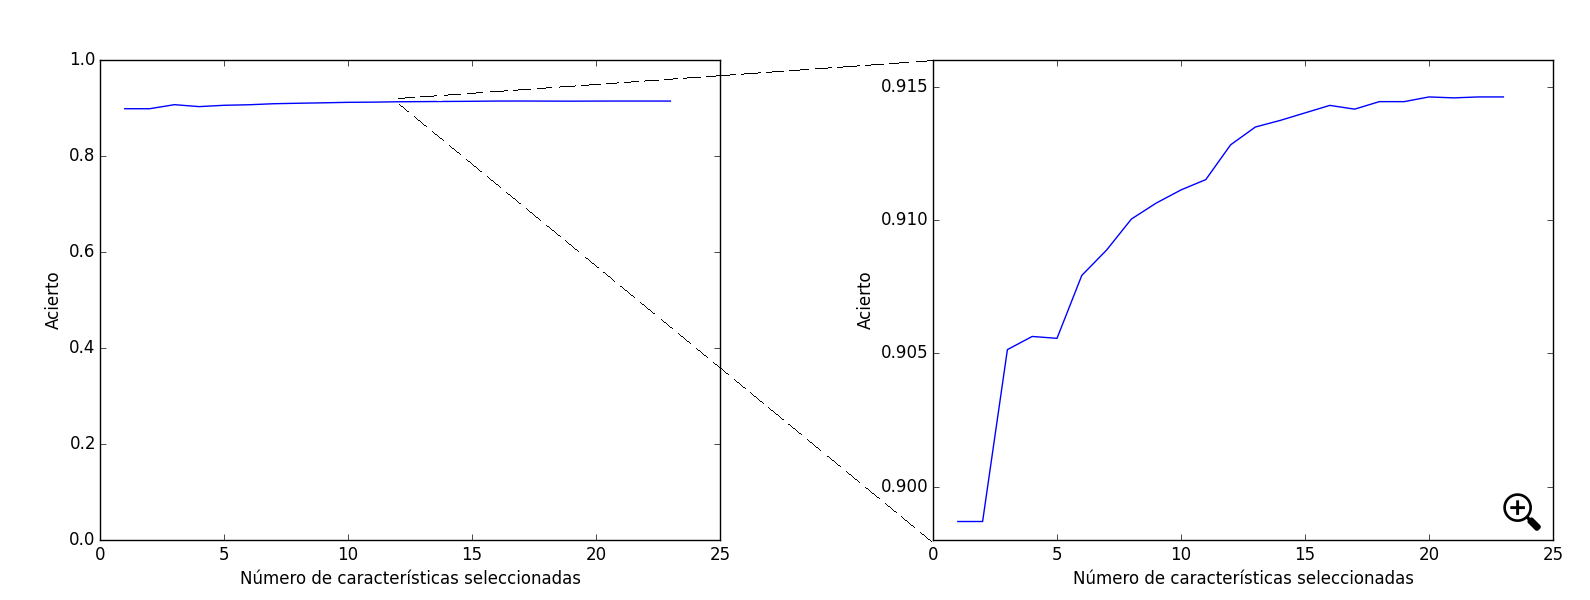
\includegraphics[height=5cm]{rfe.png}

        \vfill

        Se descartan Negación, Palabras no españolas y Antónimos
    \end{center}
\end{frame}

\subsection{Resultados obtenidos}
\begin{frame}
    \frametitle{Resultados obtenidos}

    \begin{center}
        \scriptsize
        \begin{tabular}{ c | r | r | r | r | r | r | r }
            & \multicolumn{1}{c |}{Precisión} & \multicolumn{1}{c |}{Recall} & \multicolumn{1}{c |}{$F_1$} & \multicolumn{1}{c |}{Prec. neg.} & \multicolumn{1}{c |}{Rec. neg.} & \multicolumn{1}{c |}{$F_1$ neg.} & \multicolumn{1}{c}{Acierto} \\
            \hline
            LB1 & \textbf{61,7} & \textbf{84,6} & \textbf{71,4} & \textbf{96,6} & 89,2 & 71,4 & \textbf{88,5} \\
            \hline
            LB2 & N/A & 0,0 & N/A & 83,0 & \textbf{100,0} & \textbf{90,7} & 83,0 \\
            \hline
            \hline
            SVM & 83,6 & 68,9 & \textbf{75,5} & 93,8 & 97,2 & \textbf{95,5} & \textbf{92,5} \\
            \hline
            DT & 66,5 & 67,5 & 67,0 & 93,3 & 93,0 & 93,2 & 88,9 \\
            \hline
            GNB & 57,5 & \textbf{78,2} & 66,3 & \textbf{95,2} & 88,2 & 91,5 & 86,5 \\
            \hline
            MNB & \textbf{84,8} & 60,0 & 70,3 & 92,3 & \textbf{97,8} & 95,0 & 91,4 \\
            \hline
            KNN & 81,3 & 66,3 & 73,0 & 93,4 & 96,9 & 95,1 & 91,7 \\
        \end{tabular}

        \begin{center}
            Mejor técinca: \textbf{SVM}
        \end{center}

        \begin{tabular}{ c | r | r }
            \textbf{son/clasif.} & Positivos & Negativos \\
            \hline
            Positivos & 842 & 381 \\
            \hline
            Negativos & 165 & 5805 \\
        \end{tabular}
    \end{center}
\end{frame}
\note{TODO: decir que es luego del escalado y demás}

\subsection{Otros análisis}

\subsubsection{Evaluación en el conjunto de entrenamiento}
\begin{frame}
    \frametitle{Evaluación en el conjunto de entrenamiento}

    \begin{itemize}
        \item Es una ``cota superior''
    \end{itemize}

    \begin{center}
        \scriptsize
        \begin{tabular}{ c | r | r | r | r | r | r | r }
            & \multicolumn{1}{c |}{Precisión} & \multicolumn{1}{c |}{Recall} & \multicolumn{1}{c |}{$F_1$} & \multicolumn{1}{c |}{Prec. neg.} & \multicolumn{1}{c |}{Rec. neg.} & \multicolumn{1}{c |}{$F_1$ neg.} & \multicolumn{1}{c}{Acierto} \\
            \hline
            SVM & 87,5 & 69,6 & 77,5 & 94,2 & 98,0 & 96,1 & 93,3 \\
            \hline
            DT & \textbf{100,0} & \textbf{98,8} & \textbf{99,4} & \textbf{99,8} & \textbf{100,0} & \textbf{99,9} & \textbf{99,8} \\
            \hline
            GNB & 58,1 & 77,7 & 66,4 & 95,2 & 88,8 & 91,9 & 86,9 \\
            \hline
            MNB & 84,6 & 58,9 & 69,5 & 92,3 & 97,9 & 95,0 & 91,7 \\
            \hline
            KNN & 87,0 & 71,5 & 78,5 & 94,5 & 97,9 & 96,2 & 93,5 \\
        \end{tabular}
    \end{center}
\end{frame}

\begin{frame}
    \frametitle{Evaluación en el conjunto de entrenamiento II}

    \begin{itemize}
        \item ¿Por qué DT no da 100\%? Debería darlo.
        \item Las características no discriminan completamente a la clase.
        \item ¿Hay errores en el corpus?
    \end{itemize}
\end{frame}

\begin{frame}[allowframebreaks]
    \frametitle{Inconsistencias en el corpus}

    \begin{itemize}
        \item Siguiendo la distancia mínima de edición en tweets (la granularidad es una palabra): se encontraron 367 pares de tweets ``parecidos'' pero con distinto valor de la clase objetivo.
    \end{itemize}

    \begin{example}
        Limpiar tu cuarto = 1\% limpieza. 30\% quejarse. 69\% jugar con lo que vas encontrando.
    \end{example}

    \begin{example}
        Limpiar tu cuarto:

        1\% limpieza.

        30\% quejarse.

        69\% jugar con lo que vas encontrando.
    \end{example}

    \note{
        En el primer caso son casi las mismas palabras, pero distinto espaciado y puntuación.
    }

    \framebreak

    \begin{itemize}
        \item Luego se buscan aquellos con mismos valores de atributos pero distinta clase: 30 pares encontrados.
    \end{itemize}

    \begin{example}
        \#TerminarUnaNotaDeSuicidioCon Soy Darks.
    \end{example}

    \begin{example}
        \#SiYoMeLlamaraKevinRoldan Me suicidaria.
    \end{example}
\end{frame}

\begin{frame}
    \frametitle{Inconsistencias en el corpus III}

    \begin{itemize}
        \item Hay inconsistencias en la anotación (era esperado)
        \item Hay una mejora sobre el corpus de entrenamiento, en la ``cota superior'', quitando estas instancias:

        \begin{center}
            \scriptsize
            \begin{tabular}{ c | r | r | r | r | r | r | r }
                \textbf{SVM} & \multicolumn{1}{c |}{Precisión} & \multicolumn{1}{c |}{Recall} & \multicolumn{1}{c |}{$F_1$} & \multicolumn{1}{c |}{Prec. neg.} & \multicolumn{1}{c |}{Rec. neg.} & \multicolumn{1}{c |}{$F_1$ neg.} & \multicolumn{1}{c}{Acierto} \\
                \hline
                Antes & 87,5 & 69,6 & 77,5 & 94,2 & 98,0 & 96,1 & 93,3 \\
                \hline
                Después & \textbf{89,0} & \textbf{71,3} & \textbf{79,1} & \textbf{94,7} & \textbf{98,3} & \textbf{96,5} & \textbf{94,0} \\
            \end{tabular}
        \end{center}
    \end{itemize}

    \begin{itemize}
        \item Y en el de corpus de evaluación:

        \begin{center}
            \scriptsize
            \begin{tabular}{ c | r | r | r | r | r | r | r }
                \textbf{SVM} & \multicolumn{1}{c |}{Precisión} & \multicolumn{1}{c |}{Recall} & \multicolumn{1}{c |}{$F_1$} & \multicolumn{1}{c |}{Prec. neg.} & \multicolumn{1}{c |}{Rec. neg.} & \multicolumn{1}{c |}{$F_1$ neg.} & \multicolumn{1}{c}{Acierto} \\
                \hline
                Antes & 83,6 & 68,9 & 75,5 & 93,8 & 97,2 & 95,5 & 92,5 \\
                \hline
                Después & \textbf{85,7} & \textbf{69,2} & \textbf{76,6} & \textbf{94,2} & \textbf{97,8} & \textbf{95,9} & \textbf{93,1} \\
            \end{tabular}
        \end{center}
    \end{itemize}
\end{frame}

\subsubsection{Tweets censurados}
\begin{frame}
    \frametitle{Tweets censurados}

    \begin{itemize}
        \item El clasificador está sesgado a no conocer los tweets con contenido explícito
        \item Se anotan a mano los 303 tweets censurados y se agregan
        \item Hay una pequeña mejora:
        \begin{center}
            \scriptsize
            \begin{tabular}{ c | r | r | r | r | r | r | r }
                \textbf{SVM} & \multicolumn{1}{c |}{Precisión} & \multicolumn{1}{c |}{Recall} & \multicolumn{1}{c |}{$F_1$} & \multicolumn{1}{c |}{Prec. neg.} & \multicolumn{1}{c |}{Rec. neg.} & \multicolumn{1}{c |}{$F_1$ neg.} & \multicolumn{1}{c}{Acierto} \\
                \hline
                Antes & 83,6 & 68,9 & 75,5 & \textbf{93,8} & \textbf{97,2} & \textbf{95,5} & \textbf{92,5} \\
                \hline
                Después & \textbf{84,0} & \textbf{69,6} & \textbf{76,1} & 93,7 & 97,2 & 95,4 & 92,3 \\
            \end{tabular}
        \end{center}
        \item Un nuevo estudio de importancia de las características revela que no varía Jerga sexual: se agrega más variedad que jerga sexual.
    \end{itemize}
\end{frame}

\subsubsection{Restricción a cuentas humorísticas}
\begin{frame}
    \frametitle{Restricción a cuentas humorísticas}

    \begin{itemize}
        \item Es una tarea más difícil
        \item Igualmente se logran buenos resultados:

        \begin{center}
            \scriptsize
            \begin{tabular}{ c | r | r | r | r | r | r | r }
                & \multicolumn{1}{c |}{Precisión} & \multicolumn{1}{c |}{Recall} & \multicolumn{1}{c |}{$F_1$} & \multicolumn{1}{c |}{Prec. neg.} & \multicolumn{1}{c |}{Rec. neg.} & \multicolumn{1}{c |}{$F_1$ neg.} & \multicolumn{1}{c}{Acierto} \\
                \hline
                SVM & \textbf{81,9} & 73,8 & 77,6 & 78,5 & \textbf{85,4} & \textbf{81,8} & \textbf{79,9} \\
                \hline
                DT & 74,5 & 75,5 & 75,0 & 72,2 & 71,1 & 71,7 & 74,1 \\
                \hline
                GNB & 78,7 & 78,6 & \textbf{78,6} & 76,1 & 76,3 & 76,2 & 77,5 \\
                \hline
                MNB & 68,5 & \textbf{85,5} & 76,1 & \textbf{83,3} & 64,6 & 72,9 & 74,6 \\
                \hline
                KNN & 79,2 & 73,0 & 76,0 & 77,4 & 82,9 & 80,1 & 78,1 \\
            \end{tabular}
        \end{center}
    \end{itemize}
\end{frame}

\begin{frame}
    \frametitle{Métricas ponderadas según calificación}

    \begin{itemize}
        \item Tiene sentido sólo para los tweets que tuvieron votos y para la medida recall
        \item Promedio de estrellas, $PE_t = \frac{\sum_{i = 1}^{5} i \times v_{ti}}{v_t}$
        \item $recall_{ponderado} = \frac{\sum_{t \in VP} PE_t} {\sum_{t \in VP} PE_t + \sum_{t \in FN} PE_t} = 70.68\%$
        \item $\frac{recall_{ponderado}}{recall} = \frac{prom_{VP}}{prom_H} = 1.0266$
        \item Hay un (muy) leve sesgo del clasificador SVM a dar como positivos aquellos tweets que tienen mayor promedio de estrellas.
        \item Matriz de confusión:

        \begin{center}
            \begin{tabular}{ c | r | r }
                \textbf{son/clasificados} & Humor & No humor \\
                \hline
                Humor & 2,7227 & 2,4961 \\
                \hline
                No humor & 0,0256 & 0,0300 \\
            \end{tabular}
        \end{center}
    \end{itemize}
\end{frame}

\subsubsection{Clasificación según categorías de cuentas no humorísticas}
\begin{frame}
    \frametitle{Clasificación según categorías de cuentas no humorísticas}

    \begin{center}
        \scriptsize
        \begin{tabular}{ c | r | r | r | r | r | r | r }
            \textbf{SVM} & \multicolumn{1}{c |}{Precisión} & \multicolumn{1}{c |}{Recall} & \multicolumn{1}{c |}{$F_1$} & \multicolumn{1}{c |}{Prec. neg.} & \multicolumn{1}{c |}{Rec. neg.} & \multicolumn{1}{c |}{$F_1$ neg.} & \multicolumn{1}{c}{Acierto} \\
            \hline
            Noticias & \textbf{97,0} & \textbf{95,2} & \textbf{96,1} & \textbf{97,0} & \textbf{98,1} & \textbf{97,5} & \textbf{97,0} \\
            \hline
            Reflexiones & 95,0 & 83,0 & 88,6 & 84,0 & 95,3 & 89,3 & 88,9 \\
            \hline
            Curiosidades & 94,6 & 83,7 & 88,9 & 88,2 & 96,3 & 92,1 & 90,7 \\
        \end{tabular}
    \end{center}
\end{frame}

\section{Conclusiones}

\begin{frame}
    \frametitle{Conclusiones}
    
    \begin{itemize}
        \item[\checkmark] Clasificador con 83,6\% de precisión y 68,9\% de recall
        \item[\checkmark] SVM fue el mejor
        \item[\checkmark] Diálogo característica más útil, aunque en general todas aportan algo
        \item[\checkmark] Noticias es lo que más se logra diferenciar respecto a humor
        \item[\checkmark] Se encontraron inconsistencias en la anotación
        \item[\checkmark] Características de formato y temática llevan a buenos resultados
        \item[\checkmark] Las características no discriminan completamente al humor
        \item[\checkmark] Es una tarea difícil
        \item[\checkmark] Corpus anotado
    \end{itemize}
\end{frame}

\subsection{Trabajo a futuro}
\begin{frame}
    \frametitle{Trabajo a futuro}
    
    \begin{itemize}
        \item Más características
        \item Características más complejas
        \item Regresión en el promedio de estrellas
        \item Estudiar el humor y la anotación según estratos sociales
        \item Generar humor
    \end{itemize}
\end{frame}


\begin{frame}
    \Huge{\centerline{¿Preguntas?}}
\end{frame}

\end{document}
